% --------------------
  \chapter{Diseño}
% --------------------
\label{C:diseño}

Para la etapa de diseño, se dividirá en tres partes. La primera, será el diseño eléctrico del carrito omnidireccional, con los componentes necesarios para funcionar. La segunda es el diseño del código para el carrito omnidireccional, encargado del control de los motores y la odometría de las ruedas. Por último, se hablará del diseño necesario del lado de la computadora principal, para lograr la navegación y el mapeo.

\newpage

\subsection{Carrito omnidireccional}
Para la primera etapa, se utilizará el esquema básico presentado en la figura \ref{F:diagrama}. Se requiere de un sistema que pueda controlar los motores, y además llevar control de la odometría de las ruedas. Además se deberá incorporar el sensor de profundidad en el carrito omnidireccional.

\begin{figure}[H]
\centering
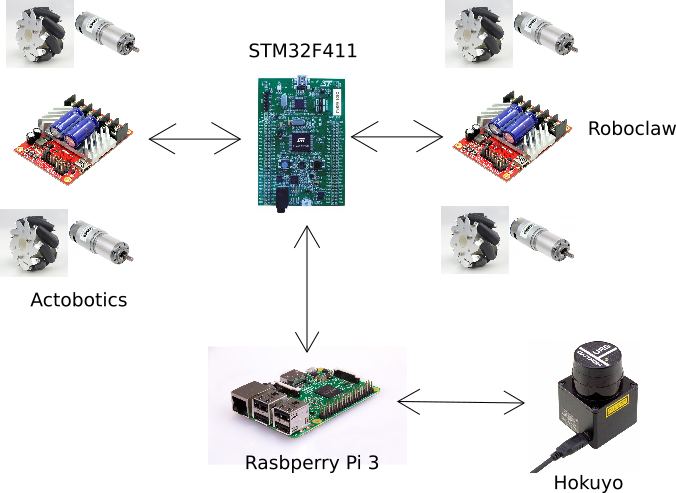
\includegraphics[scale=0.6]{imagenes/diagrama_diseno.png}
\caption{Diagrama básico de la implementación de la parte elétrica del carrito omnidireccional. Autoría propia.}
\label{F:diagrama}
\end{figure}

Empezando por los \textbf{motores}, se utilizarán motores DC Actobotics 638276. La hoja de fabricante con los datos en la sección de los apéndices. Además, en la tabla \ref{T:actobotics} se muestra la información más relevante de los motores a utilizar, como por ejemplo el consumo máximo, la tensión de trabajo, y la relación de los engranes.

\begin{table}[H]
\caption{Información más relevante de los motores Actobotics, a ser utilizados. Autoría propia.}
\begin{tabular}{|l|l|}
\hline
Especificación                & Valor         \\ \hline
Voltage de operación          & 6-12 VDC      \\ \hline
Corriente máxima de operación & 0.53 A        \\ \hline
Velocidad máxima sin carga    & 118 $\pm$ 12 rpm \\ \hline
Corriente máxima detenido     & 20 A          \\ \hline
Razón de los engranes         & 1/71          \\ \hline
Clicks del encoder por revolución & 3408      \\ \hline
\end{tabular}
\label{T:actobotics}
\end{table}

Se utilizarán cuatro motores, uno para cada rueda, conectados a ruedas mecanum genericas, de 6mm de diámetro. Estas son ruedas omnidireccionales con rodillos a un ángulo de $\alpha = 45^\circ$.

En lo que concierne a los \textbf{controladores} de los motores, no se diseñarán, puesto que se utilizarán controladores comerciales de marca IonMotion Roboclaw. En específico, se utilizará el modelo Roboclaw 2x15A. En el cuadro \ref{T:roboclaw} se resumen los datos más importantes de este controlador.

\begin{table}[H]
\caption{Información más relevante de los controladores Roboclaw 2x15A. Autoría propia.}
\begin{tabular}{|l|l|}
\hline
Especificación                      & Valor          \\ \hline
Tensión de la batería principal     & 6-34 VDC       \\ \hline
Tensión de la batería lógica        & 6-34 VDC       \\ \hline
Bits de los contadores para encoder & 32 bits        \\ \hline
Velocidad máxima sin carga          & 118 +- 12 rpm  \\ \hline
R232 Baud Rate                      & 460,800 Bits/s \\ \hline
Tensión de I/O                      & 3.3 VDC        \\ \hline
\end{tabular}
\label{T:roboclaw}
\end{table}

Es importante mencionar, que estos controladores se utilizan para manejar los motores. Pueden manejar hasta dos motores, y son muy versátiles en cuánto a cómo se pueden utilizar. En particular, para este proyecto se usará la comunicación serial que posee el controlador. En la figura \ref{F:roboclaw} se muestran los pines que posee el roboclaw. En específico, los pines S1, y S2 se pueden utilizar como puertos USART para comunicación serial. La tabla \ref{T:pines} muestra las funcionalidades que pueden cumplir cada pin.

\begin{figure}[H]
\centering
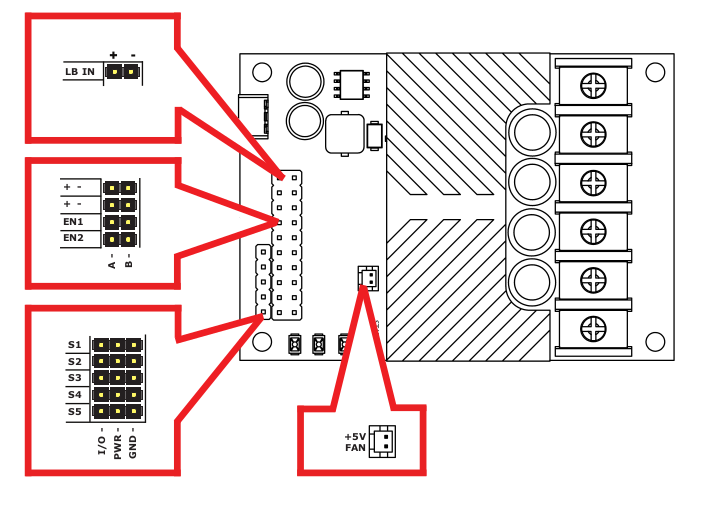
\includegraphics[scale=0.5]{imagenes/roboclaw.png}
\caption{Muestra de los pines de un Roboclaw 2x15A fabricado por IonMotion. Tomado del manual del fabricante.}
\label{F:roboclaw}
\end{figure}

\begin{table}[H]
\centering
\caption{Tabla con las funciones de los pines en un Roboclaw 2x15A fabricado por IonMotion. Tomado del manual del fabricante.}
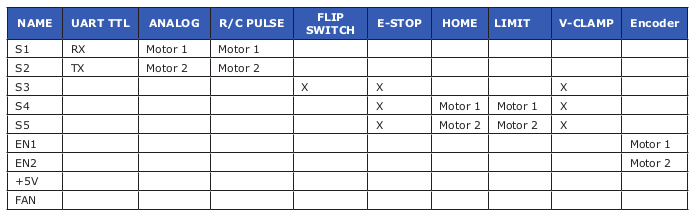
\includegraphics[scale=0.7]{imagenes/pines.png}
\label{T:pines}
\end{table}

Se utilizará una frecuencia de 115200 en la transmisión serial, ya que es la más alta soportada por el dispositivo. En el modo llamado ``Packet Serial'', el cuál funciona mediante el protocolo RS-232 para controlar la dirección y velocidad de cada uno de los motores.

El fabricante da ejemplo de código que se puede utilizar para enviar comandos, y especifica el protocola utilizado en el manual de usuario. Todas las instrucciones utilizan un checksum crc16bit para verificación de las intrucciones.

Siguiendo el esquema de la figura \ref{F:diagrama}, los controladores Roboclaw van conectados al \textbf{microcontrolador} STM32F411. La principal función de este microcontrolador será llevar cuenta de la odometría de cada una de las ruedas, y del robot como tal. Además, este aceptará instrucciones por USB del Raspberry Pi, de movimiento en el formato $(V_X, V_Y, W_Z)$ y enviará información de vuelta de la odometría del robot en el formato $(X_X, X_Y, \alpha_Z)$. También enviará instrucciones de movimiento a los dos controladores Roboclaw, y controlará la velocidad de cada motor por medio de un PID, en lazo cerrado con la información del encoder como entrada.

El esquema mostrado en la figura \ref{F:diagrama_stm} muestra en resumen lo que se explicó anteriormente.

\begin{figure}[H]
\centering
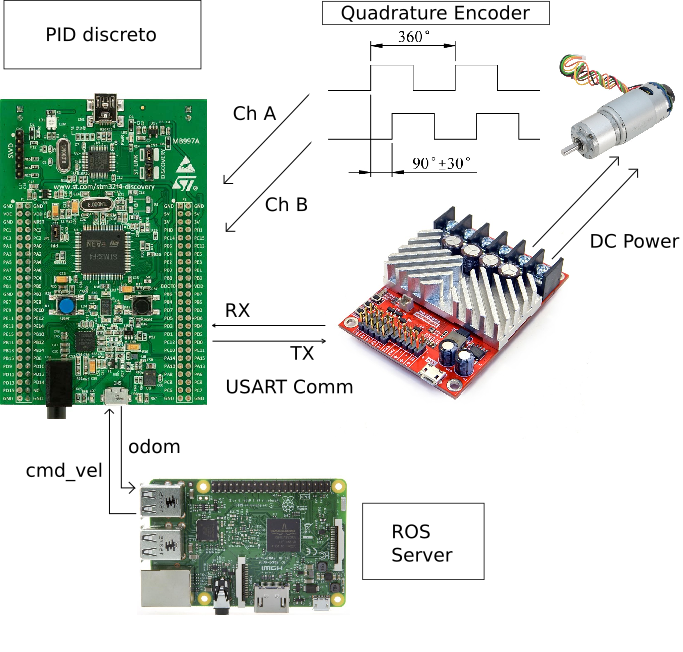
\includegraphics[scale=0.5]{imagenes/microcontrolador_diagrama.png}
\caption{Diagrama de las funciones que debe realizar el microcontrolado STM32F411. Autoría propia.}
\label{F:diagrama_stm}
\end{figure}

Es importante notar, que la programación del microcontrolador se realizará mediante las liberías libopencm3 y libopencm3-plus, las cuáles permiten escribir el código en el lenguaje de programación C. Además, el microcontrolador posee las funciones para leer los encoders directamente, puesto que posee timers que se pueden configurar en un modo para leer codificadores de cuadratura.

Información sobre el uso de encoders de cuadratura en el stm se puede encontrar en apéndice correspondiente.

Finalmente, un diagrama de las conexiones eléctricas se puede encontrar en la figura \ref{F:conexiones}. En este diagrama se incluye la información de los pines pertinentes en cada dispositivo.

\begin{figure}[H]
\centering
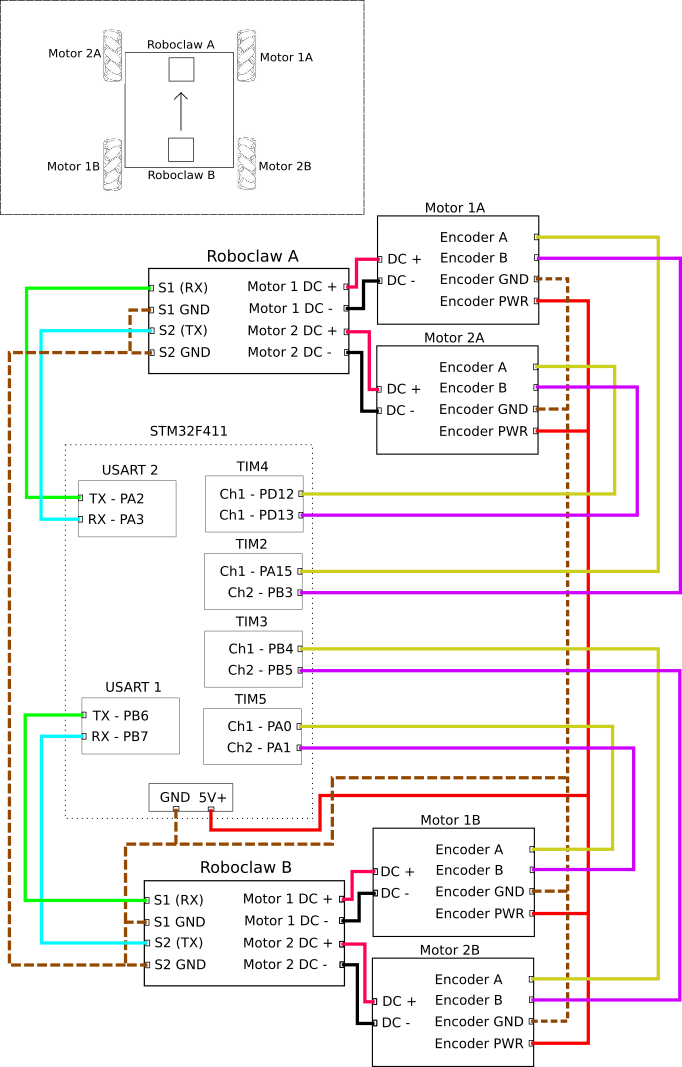
\includegraphics[scale=0.63]{imagenes/diagrama_electrico.png}
\caption{Diagrama de las conexiones eléctricas entre los dispositivos. Autoría propia.}
\label{F:conexiones}
\end{figure}

\subsection{Código}




\newpage

El capítulo 3 y los subsiguientes (si fueran necesarios), mostrarán el trabajo realizado en el proyecto, por lo que su cantidad, títulos y divisiones, se dejan a discreción del estudiante, con la aprobación del profesor guía y demás miembros de Tribunal evaluador.

Estos capítulos muestran el ``producto'' del trabajo realizado en el proyecto, por lo cual constituyen la parte medular del informe. Debe explicarse en forma clara, qué se hizo, cómo se hizo y qué se obtuvo.

Cuando se agregan o remueven del texto elementos que aparecen en los índices (general, de figuras, de cuadros) que están en el preámbulo del informe, así como cuando se agregan o remueven citas a las fuentes bibliográficas, que aparecen en la Bibliografía al final del documento, es necesario ejecutar dos o tres veces la compilación del documento, para que estas listas se confeccionen nuevamente y se muestren correctamente.  También, en el caso de agregar o quitar ecuaciones, es necesario recompilar dos o tres veces el documento, para que se renumeren las ecuaciones y  las referencias a estas.

\begin{equation}
x_{1,2} = \frac{-b \pm \sqrt{b^2 - 4ac}}{2a}
\end{equation}

\section{Manejo de las fuentes bibliográficas}
Cuando se realiza un trabajo de desarrollo o investigación, siempre se parte del trabajo realizado por otras personas. Es por lo tanto indispensable, hacer referencia a las fuentes bibliográficas (referencias) utilizadas.

En \LaTeX se utiliza BibTeX para el manejo de la bibliografía.  La información de las fuentes consultadas (libros, artículos de revista o ponencias en congresos, tesis, etc.), se almacenan en un archivo \texttt{.bib} (base de datos de las fuentes bibiográficas), sin preocuparse del formato en que estas serán mostradas en el informe.  Para la creación y manejo de este archivo, se puede utilizar el programa JabRef\footnote{http://jabref.sourceforge.net/} o uno similar.

La forma en que las fuentes son listadas en el apartado Bibliografía, y como son mostradas en el texto cuando se citan, depende del \emph{estilo} seleccionado para esto.

\begin{equation}
Z = \begin{cases}
\sqrt{\epsilon_r - \cos^2 \theta}/\epsilon_r & \text{para polarización vertical} \\
\sqrt{\epsilon_r - \cos^2 \theta} & \text{para polarización horizontal} \\
\end{cases}
\end{equation}

Para el informe del proyecto eléctrico, se debe utilizar el formato APA\footnote{American Psychological Association, http://www.apa.org/}.  En inglés, este se establece utilizando el estilo \texttt{apalike}.

\begin{equation}
 e^{jx} = \cos{x} + j \sin{x}
\end{equation}

Junto con la clase \texttt{eieproyecto} se suministra el archivo de estilo de bibliografía \texttt{apalike\_es.bst}, en el cual se han cambiado los términos en ingles (ej. ``and'', ``In'', Edition y otros) por su equivalente en español.  Este archivo debe colocarse en la misma carpeta, en donde están los demás archivos utilizados para la confección del informe.

\begin{equation}
\int_0^\infty e^{-x^2} \mathrm{d}x = \frac{\sqrt{\pi}}{2}
\end{equation}

\begin{equation}
\mathbb{A-Z} \quad
\mathcal{A-Z}
\end{equation}

Por lo tanto, la lista de las fuentes bibliográficas utilizadas se confecciona automáticamente, a partir de las citas hechas en el texto.  Solo las fuentes citadas aparecerán en la bibliografía.

\begin{equation}
u(x) =
  \begin{cases}
   \exp{x} & \text{si } x \geq 0 \\
   1       & \text{si } x < 0
  \end{cases}
\end{equation}

Como se indicó anteriormente, se emplean \texttt{cite} y \texttt{citep} para hacer las citas.  Cual de estos dos comandos conviene utilizar, dependerá del contexto en que se haga la cita.  Según la redacción del párrafo, puede convenir que la fuente se indique en el formato ``Autor (año)'', pero en otros casos pudiera ser preferible que esta aparezca en el formato ``(Autor, año)''.

\begin{equation}
r(t) = \Re \left\lbrace \frac{\lambda}{4\pi} \left[ \frac{\sqrt{G_0} u(t) e^{-j2\pi r_0/\lambda}}{r_0} + \frac{\Gamma \sqrt{G_1} u(t-\tau) e^{-j2\pi r_1/\lambda}}{r_1} \right] e^{j2\pi f_c t}  \right\rbrace
\end{equation}
